\documentclass{article}
\PassOptionsToPackage{sort,numbers,square}{natbib}

\usepackage{nips_2018}
\usepackage[utf8]{inputenc} % allow utf-8 input
\usepackage[T1]{fontenc}    % use 8-bit T1 fonts
\usepackage{hyperref}       % hyperlinks
\usepackage{url}            % simple URL typesetting
\usepackage{booktabs}       % professional-quality tables
\usepackage{amsfonts}       % blackboard math symbols
\usepackage{nicefrac}       % compact symbols for 1/2, etc.
\usepackage{microtype}      % microtypography

% For citations
\usepackage{natbib}

% For algorithms
\usepackage{algorithm}
\usepackage{algorithmic}
\usepackage{hyperref}
\hypersetup{backref,colorlinks=true,citecolor=blue,linkcolor=blue,urlcolor=blue}

%\newcommand{\theHalgorithm}{\arabic{algorithm}}


\usepackage{graphicx}
\usepackage{subfigure} 
%\graphicspath{{../nips-2018/}}


%Arash
\usepackage{amsmath,amsthm}
\usepackage{amssymb}
\usepackage{mathrsfs}
\DeclareMathOperator*{\argmin}{argmin}
\usepackage{siunitx}
\usepackage{comment}
\usepackage{mathtools}
\mathtoolsset{showonlyrefs}

\renewcommand*{\figureautorefname}{}%
\renewcommand*{\tableautorefname}{Table}%
\renewcommand*{\sectionautorefname}{Section}%
\renewcommand*{\subsectionautorefname}{Section}%
\renewcommand*{\subsubsectionautorefname}{Section}%

\newtheorem{theorem}{Theorem}%[section]
\newtheorem{definition}[theorem]{Definition}
\newtheorem{lemma}[theorem]{Lemma}



\usepackage{gensymb}
\usepackage{xcolor}
\newcommand{\attn}[1]{\textcolor{red}{TODO: #1}}
\newcommand{\one}{\mathbf{1}}
\renewcommand{\algorithmiccomment}[1]{\hfill $\rhd$ #1}
\newcommand{\given}{\;\vert\;}
\newcommand*{\algorithmautorefname}{Algorithm}%
\newcommand{\norm}[1]{\left\lVert #1 \right\rVert}
\DeclareMathOperator*{\prox}{\bf prox}
\DeclareMathOperator*{\sign}{sign}

\usepackage{xr}
\externaldocument{paper}



\title{Supplement for "Modeling trend in temperature volatility using generalized LASSO"}

\author{Arash Khodadadi\\
 Department of Statistics\\
 Indiana University\\
 Bloomington, IN 47408 \\
 \texttt{arakhoda@indiana.edu}
\And
  Daniel J.\ McDonald \\
 Department of Statistics\\
 Indiana University\\
 Bloomington, IN 47408 \\
 \texttt{dajmcdon@indiana.cmu.edu}}


\begin{document} 


\maketitle

\section{Appendix A}
\label{sec:app_l1tf_var}

In this appendix we provide more details on how to solve the optimization problem \ref{eq:l1tf_var} using PDIP. The objective function is convex but not differentiable. Therefore, to be able to use PDIP we first need to derive the dual of this problem. We note that this is a generalized LASSO problem \citep{tibshirani_solution_2011}. The dual of a generalized LASSO with the objective $f(x)+\lambda \norm{ Dx }_1$ is:  

\begin{align}
\min_\nu&\quad f^*(-D^\top\nu) & \mbox{s.t.}&\quad \norm{ \nu }_\infty \le \lambda
\end{align}

where $f^*(\cdot)$ is the Fenchel conjugate of $f$: $f^*(u)=\max_x u^\top x-f(x)$. It is simple to show that 

\begin{equation}
f^*(u)=\sum_t (u_t-1)\log\frac{y_t^2}{1-u_t} + u_t-1.
\label{eq:conj}
\end{equation}

Each iteration of PDIP involves computing a search direction by taking a Newton step for the system of nonlinear equations $r_w(v,\mu_1,\mu_2)=0$, where $w>0$ is a parameter and

\begin{equation}
  r_w(v,\mu_1,\mu_2):=
	\begin{bmatrix}
	r_{dual}\\
	r_{cent}	
	\end{bmatrix}=
  \begin{bmatrix}
    \nabla f^*(-D^\top v) + \mu_1 - \mu_2\\
    -\mu_1(v-\lambda\one)+\mu_2(v + \lambda\one) -w^{-1}\one
  \end{bmatrix}
\label{eq:resid}
\end{equation}

for $w>0$, where $\mu_1$ and $\mu_2$ are dual variables for the $\ell_\infty$ constraint. Let $A=[\nabla r_{dual}^\top , \nabla r_{cent}^\top]^\top$. The newton step takes the following form

\begin{equation}
r_w(v,\mu_1,\mu_2)+A
\begin{bmatrix}
	\nabla v\\
	\nabla \mu_1\\
	\nabla \mu_2	
	\end{bmatrix}= 0
\label{eq:newton_step}
\end{equation}


We have:

\begin{equation}
A=
\begin{bmatrix}
	\nabla^2 f^*(-D^\top v) & I & -I\\
	-\mathbf{diag(\mu_1)}\one & -v+\lambda\one & \mathbf{0}\\
	\mathbf{diag(\mu_2)}\one & v+\lambda\one & \mathbf{0}
	\end{bmatrix}
\label{eq:delta_r}
\end{equation}

Therefore, to perform the Newton step we need to compute $\nabla f^*(-D^\top v)$ and $\nabla^2 f^*(-D^\top v)$. It is straightforward to show that

\begin{align}
\nabla f^*(-D^\top v) = -\nabla_u f^*(u) D^\top ,\quad u=-D^\top v, \quad (\nabla_u f^*(u))_j=\log\bigg(\frac{y_j^2}{1-u_j}\bigg) \\
\nabla^2 f^*(-D^\top v)=D\nabla_u^2 f^*(u)D^\top, \quad (\nabla_u^2 f^*(u))_j=\mathbf{diag}\bigg(\frac{1}{1-u_j}\bigg)
\end{align}


\section{Appendix B}
\label{sec:app_consADMM}

In this Appendix we give more details on performing the x-update step in \autoref{eq:ADMM_steps}. We need to solve the following optimization problem:

\begin{equation}
\hat{x}:=\argmin_{x} \bigg( \sum_{j=1}^{n_b} (x_j + y_j^2e^{-x_j}) + (\rho/2) \lVert x-\tilde{z} + u \lVert_2^2 + \Lambda^\top |D x| \bigg)
\label{eq:x_update_opt}
\end{equation}

\noindent where $n_b$ is the number of local variables in each sub-cube in \autoref{fig:data_cube}, and for ease of notation we have dropped the subscript $i$ and superscript $m$. Let $f(x)=\sum_{j=1}^{n_b} (x_j + y_j^2e^{-x_j}) + (\rho/2) \lVert x-\tilde{z} + u \lVert_2^2$. As it was explained in \autoref{sec:l1tf_var}, the dual of this optimization problem is: $\min_\nu f^*(-D^\top\nu)$ with the constraints $|\nu_k| \le \Lambda_k$. So to use PDIP we first need to compute the conjugate function $f^*(\cdot)$. We have:


\begin{align}
f^*(\xi) & = \max_x \quad \xi^\top x - f(x)\\
& =  \max_x \quad \sum_{j=1}^{n_b} (\xi_jx_j - x_j - y_j^2e^{-x_j} - (\rho/2)(x_j-\tilde{z}_j+u_j))
\label{eq:conjugate}
\end{align}

Setting the derivative of the terms inside the summation to 0, we obtain:

\begin{equation}
\xi_j-y_j^2e^{-x_j^*}-\rho x_j^* + \rho (\tilde{z}_j-u_j)=0
\label{eq:x_start}
\end{equation}

\noindent where $x^*$ is the maximizer in \ref{eq:conjugate}. Then, it can be shown that $x_j^*$ which satisfies \eqref{eq:x_start} can be obtained as follows:

\begin{align}
x^*_j & = \mathscr{W}\bigg(\frac{y_j^2}{\rho} e^{\phi_j} \bigg) - \phi_j \\
\phi_j & =\frac{1-\xi_j-\rho(\tilde{z}_j-u_j)}{\rho}
\end{align}

In this equation, $\mathscr{W}(\cdot)$ is the \textit{Lambert function} \cite{corless_lambertw_1996}. Finally, the conjugate function is: $f^*(\xi) = \sum_{j=1}^{n_b} (\xi_jx^*_j - x^*_j - y_j^2e^{-x^*_j} - (\rho/2)(x^*_j-\tilde{z}_j+u_j))$.

To use PDIP, we also need to evaluate $\nabla f^*$ and $\nabla^2 f^*$. First note that $\frac{\partial \mathscr{W}(q)}{\partial q} = \frac{\mathscr{W}(q)}{q(1+\mathscr{W}(q))}$ and $\frac{\partial^2 \mathscr{W}(q)}{\partial q^2} = - \frac{\mathscr{W}^2(q)(\mathscr{W}(q)+q)}{q^2(1+\mathscr{W}(q))^3}$. Using the chain rule we get:

%\x^*_j + \xi_j + \frac{\partial \x^*_j}{\partial \xi_j}

\begin{equation}
\frac{\partial f^*(\xi)}{\partial \xi_j}  =  x^*_j  + \frac{\partial x^*_j}{\partial \xi_j} \bigg[ \xi_j -1 + y_j^2 e^{-x_j^*} + \rho (\tilde{z}_j - u_j - x_j^*) \bigg]
\label{eq:d_f*_start}
\end{equation}
where we have:

\begin{equation}
\frac{\partial x_j^*}{\partial \xi_j}  = \frac{1}{\rho(1+\mathscr{W}((y_j^2/\rho) e^{-\phi_j} ))}
\label{eq:d_x*_start}
\end{equation}

By some tedious but straightforward computation we can obtain the second derivatives:


\begin{align}
\frac{\partial^2 f^*(\xi)}{\partial \xi_j^2} & =  \frac{\partial x_j^*}{\partial \xi_j} - \rho \frac{\partial^2 x_j^*}{\partial \xi_j^2} \bigg[ \phi_j +x_j^* - \tilde{z}_j + u_j \bigg]\\
& \quad + \frac{\partial x_j^*}{\partial \xi_j} \bigg[ 1-y_j^2 \frac{\partial x_j^*}{\partial \xi_j} e^{-x_j^*} -\rho \frac{\partial x_j^*}{\partial \xi_j} \bigg]
\label{eq:d2_f*_start}
\end{align}


\begin{equation}
\frac{\partial^2 x_j^*}{\partial \xi_j^2}  = \frac{\mathscr{W}((y_j^2/\rho) e^{-\phi_j} )}{\rho^2(1+\mathscr{W}((y_j^2/\rho) e^{-\phi_j} ))^3}
\label{eq:d2_x*_start}
\end{equation}

Having computed the conjugate function and its gradient and Jacobian, now we can use a number of convex optimization software packages which have an implementation of PDIP to perform the x-update step inside the ADMM loop. We chose the python API of the \texttt{cvxopt} package ~\citep{andersen_cvxopt:_2013}. 

\section{Appendix C}
\autoref{tab:sim_params} lists the parameters used for simulating data
in \autoref{sec:simulations}. \autoref{fig:true_var_spatial} shows the
variance function obtained from there parameters at $t=25$ (left) and
$t=45$ (center). 

\begin{table}[tb]
  \caption{Parameters used to simulate data. \attn{Any ideas to take
      up less space with this info?}}
  \label{tab:sim_params}
  \begin{center}
    \begin{tabular}{ccccccc}
      \hline
      $s$ & $r_s$ & $c_s$ & $\sigma_s$ &$\alpha_s$ & $\omega_s$ & $\phi_s$\\
      \hline
      1 & 0 & 0 & 5 & 0.5 & 0.121 & 0 \\
      2 & 0 & 5 & 5 & 0.1 & 0.121 & 0 \\
      3 & 3 & 0 & 5 & -0.5 & 0.121 & $\pi/2$ \\
      4 & 3 & 5 & 5 & -0.1 & 0.121 & $\pi/2$ \\
      \hline
    \end{tabular}
  \end{center}
\end{table} 

\begin{figure}[tb]
  \centering	
  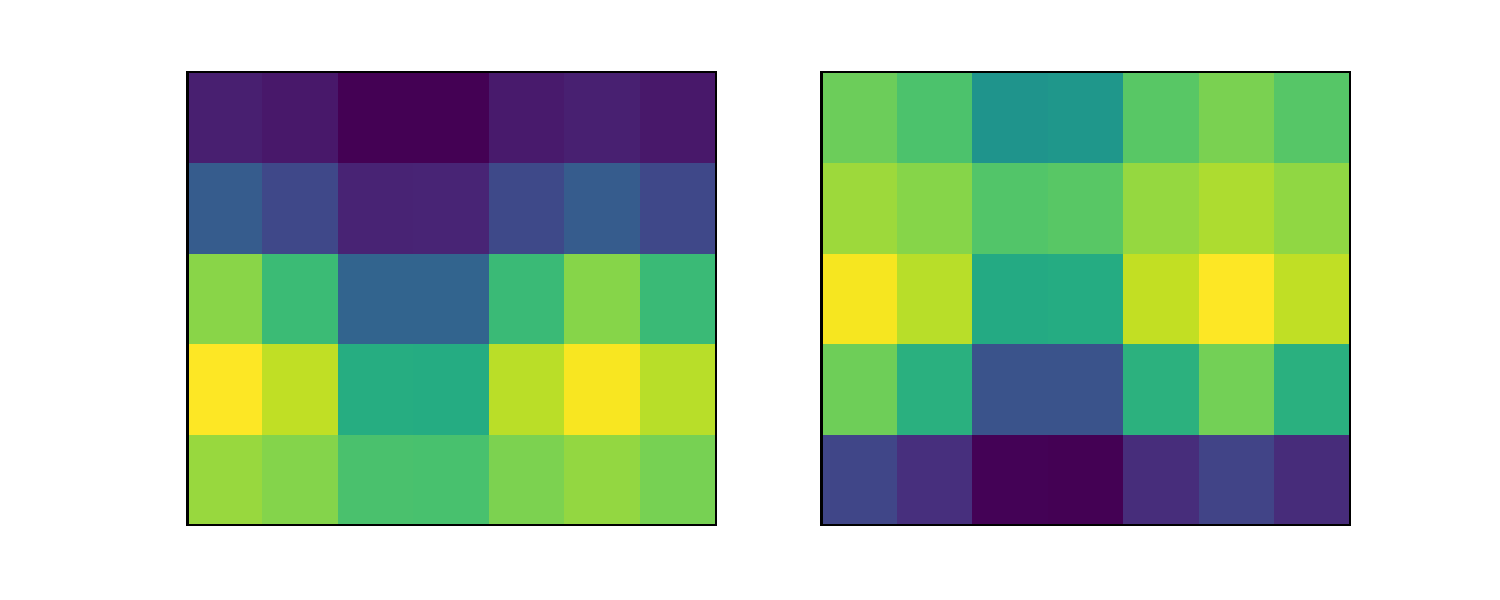
\includegraphics[height=.15\textheight]{Figures/true_var_spatial}
  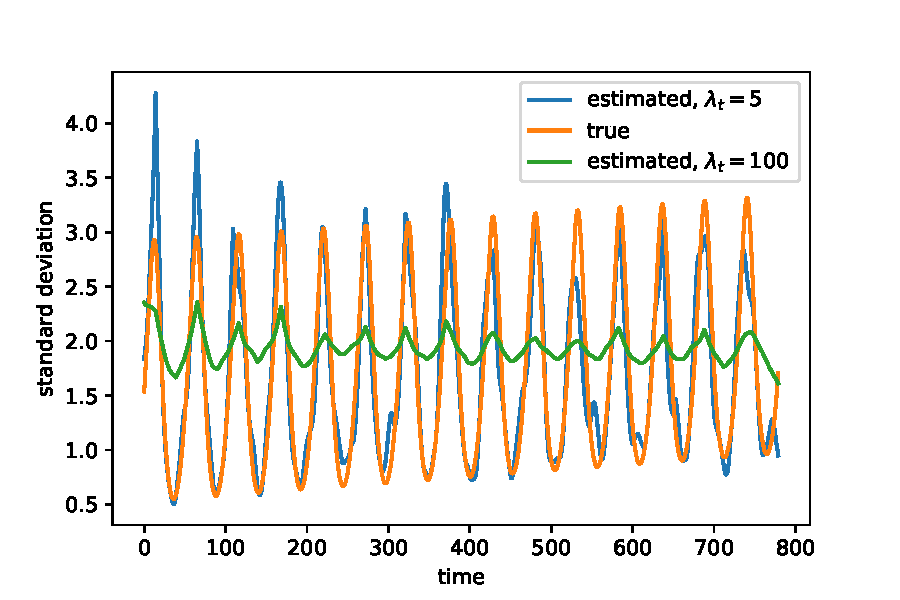
\includegraphics[height=.15\textheight]{Figures/true_fitted_var}
  \caption{Variance function at $t=25$ (left) and $t=45$
    (center). Right: the true (orange) and estimated standard deviation 
    function at the location (0,0). The estimated values are
    obtained using linearized ADMM with $\lambda_s=0.1$ and two
    values of $\lambda_t$: $\lambda_t=5$ (blue) and
    $\lambda_t=100$ (green).} \label{fig:true_var_spatial}
\end{figure}

\section{Appendix D}

In this appendix we examine some of the properties of the time-series of the temperature in ERA-20C dataset. The goal here is to demonstrate some of the difficulties in modeling the trend in the temperature volatility and motivate our methodology.

\autoref{fig:cities_ts} shows the time-series of the temperature of three cities: Bloomington (USA), San Diego (USA) and Manaus (Brazil). The time-series of Bloomington and San Diego show clear cyclic behavior. However, while it seems (qualitatively) that these cycles can be modeled by a sinusoidal function for Bloomington, the same is not true for San Diego. Also, the amplitude of the cycles changes from some years to others. The time-series of Manaus does not show any regular cyclic behavior. This demonstrates the first difficulty in analyzing the variance of this data: to analyze the variance, we first need to remove the cyclic terms from all time-series. However, there is a lot of variations in the cyclic behavior of the time-series of different locations. In addition, some of these cycles cannot be easily modeled by a parametric function \footnote{One might try to model the cycles by the summation of sinusoidal terms with different frequencies. However, for some time-series this may need many terms to be included in the summation to achieve a reasonable level of accuracy. In addition, this model cannot capture the non-stationarity in the cycles.}. To overcome these issues, we use a non-parametric approach to remove the cyclic terms from the time-series and de-trend them. This approach, called \textit{$\ell_1$-trend filtering} is explained in Section 2 of the text. We detrended each time-series separately using this method. For each time-series, we found the optimal value of the penalty parameter using \textit{k-fold cross-validation} with $k=5$. We used the R package \textbf{genlasso} to perform these computations \cite{arnold_efficient_2016}. 


\begin{figure}[tb]
	\centering
	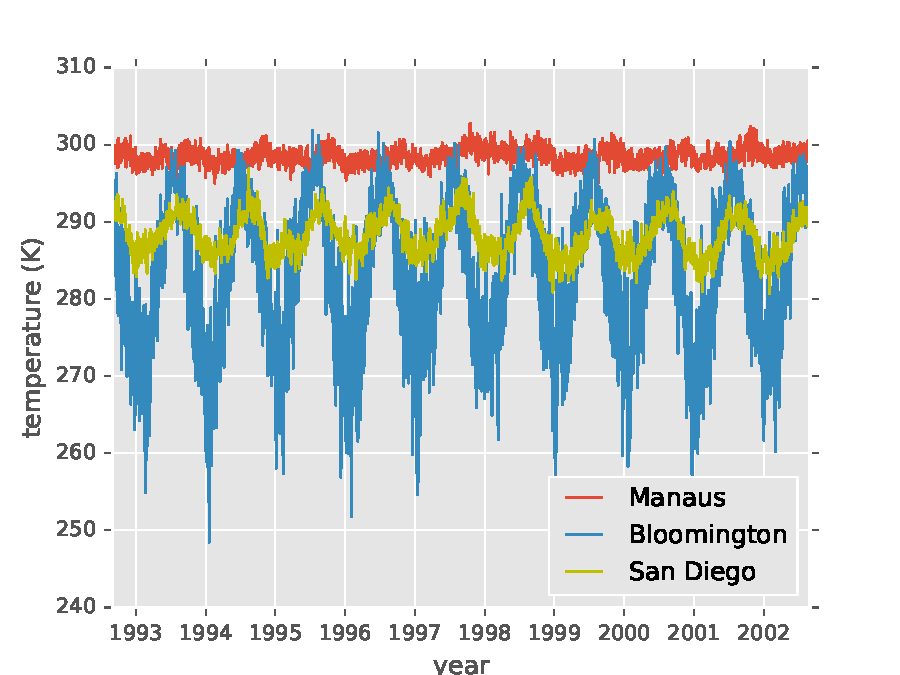
\includegraphics[width=.2\textheight]{Figures/cities_ts}
 	\caption{Time-series of the temperature (in Kelvin) of three cities.}
 	\label{fig:cities_ts}
\end{figure} 

The blue curve in the left panel of \autoref{fig:bloom_estimatedSD} shows the time-series of the temperature of Bloomington after detrending using this method. This figure, reveals another difficulty in estimating the trend of volatility in this data: the variance of this signal, shows cyclic behavior. Also, the cycles are not regular and their amplitude and frequency change. Even if one can describe the behavior of the variance of the time-series at all locations using a single parametric model (for example a variant of the GARCH models \citep{bollerslev_generalized_1986}), it is not clear how the trend in the variance should be investigated in this framework. These observations motivate the need to develop a non-parametric framework for the problem at hand.

\begin{figure}[tb]
  \centering
  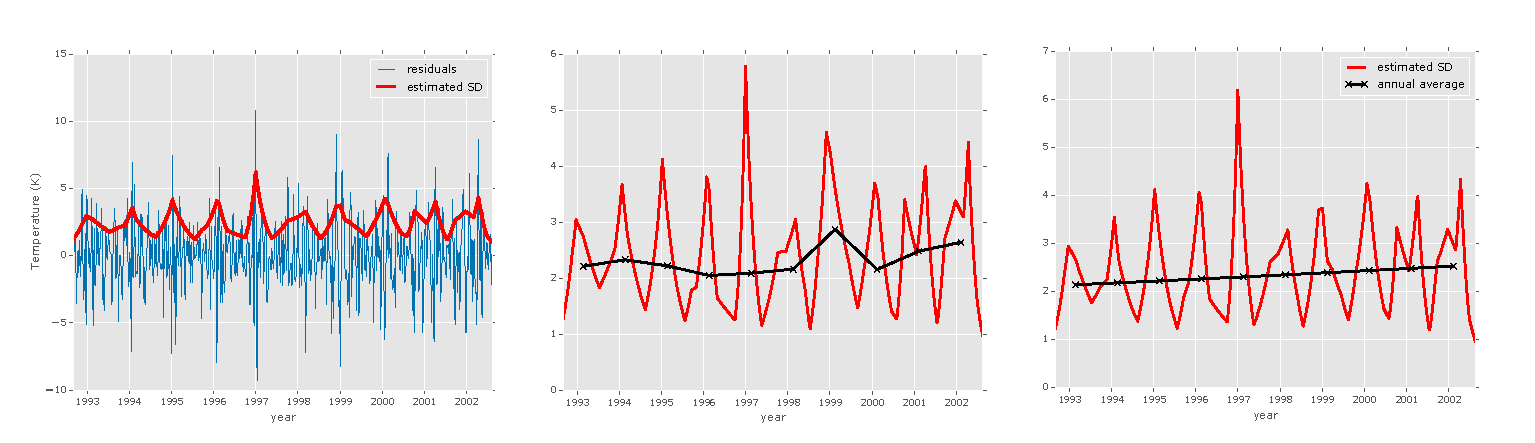
\includegraphics[width=\columnwidth]{Figures/bloom_estimatedSD}
  \caption{Left: The residuals of the time-series of Bloomington
    (averaged weekly) and the estimated SD obtained from the method of
    \autoref{sec:l1tf_var} (red). Middle: the estimated SDs (red) and
    their annual average (black) without imposing the long horizon
    penalty. Right: the same as middle panel but here the long horizon
    penalty is imposed. See the text for more details.} 
  \label{fig:bloom_estimatedSD}
\end{figure} 


The red curve in the left panel of \autoref{fig:bloom_estimatedSD}
shows the estimated SD (which is $\exp(h_t/2)$) of the residuals of
the time-series of Bloomington obtained from out proposed model. To reduce the number of time-steps we work on the weekly averaged of the data. The curve of the estimated SD captures the periodic variations in the
SD of the signal. Just by looking at this curve, it is hard to say if
the SD is decreasing or increasing. Therefore, we compute the average
of the estimated SD for each year. The estimated SD together with this
annual average is shown in the middle panel of
\autoref{fig:bloom_estimatedSD}. As it can be seen, the annual trend
is not smooth. This is because in the optimization problem
\eqref{eq:l1tf_var}, the smoothness of the annual trend is not
encouraged. To remedy this, we add the following long horizon penalty to \eqref{eq:l1tf_var}:
 
\begin{equation}
\sum_{i=1}^{N_{year}-2} \Big\arrowvert \sum_{t=1}^{52} h_{t_1}-2h_{t_2}+h_{t_3}  \Big\arrowvert
\label{eq:lh_penalty}
\end{equation}

where $t_1=52(i-1)+t$, $t_2=52i+t$ and $t_3=52(i+1)+t$. Also,
$N_{year}$ is the number of years over which we are performing our
analysis (here $N_{year}=10$). Since we are working on the weekly
averaged data, each year corresponds to 52 observations. In the matrix
form, the penalty \eqref{eq:lh_penalty} adds $N_{year}$ rows to the
matrix $D$. The estimated SDs using this penalty matrix is shown in
the right panel of \autoref{fig:bloom_estimatedSD}. The annual average
of the estimated SDs shows a linear trend with a positive slope. 

\bibliographystyle{abbrvnat}
\small
\bibliography{nips-references}


\end{document}